% Istos — Senior Engineer Field Manual (rich edition)
% Compile from this directory:
%   pdflatex learning.tex && pdflatex learning.tex
%   (or: latexmk -pdf learning.tex)
\documentclass[11pt,a4paper]{article}

\usepackage[margin=2.1cm]{geometry}
\usepackage{microtype}
\usepackage{booktabs}
\usepackage{longtable}
\usepackage{array}
\usepackage{tabularx}
\usepackage{multirow}
\usepackage{enumitem}
\usepackage{hyperref}
\usepackage{xcolor}
\usepackage{listings}
\usepackage{fancyhdr}
\usepackage{titlesec}
\usepackage{tcolorbox}
\usepackage{tikz}
\usepackage{graphicx}
\usetikzlibrary{arrows.meta,positioning,shapes.geometric,fit,calc}

\tcbuselibrary{skins,breakable}

\hypersetup{
  colorlinks=true,
  linkcolor=black,
  urlcolor=blue!50!black,
  citecolor=black,
  pdftitle={Istos Senior Engineer Field Manual},
  pdfauthor={Istos learning notes}
}

\definecolor{istosblue}{RGB}{36,99,155}
\definecolor{istoswarn}{RGB}{160,90,20}
\definecolor{istosok}{RGB}{30,110,70}
\definecolor{istoscode}{RGB}{245,246,248}

\lstdefinestyle{istos}{
  basicstyle=\ttfamily\footnotesize,
  breaklines=true,
  frame=single,
  rulecolor=\color{black!20},
  framesep=5pt,
  xleftmargin=0.4em,
  xrightmargin=0.4em,
  backgroundcolor=\color{istoscode},
  keywordstyle=\bfseries\color{istosblue},
  commentstyle=\itshape\color{black!45},
  stringstyle=\color{istosok},
  showstringspaces=false,
  columns=fullflexible,
  keepspaces=true,
  tabsize=4,
  language=Python
}
\lstset{style=istos}

\newtcolorbox{keybox}[1][]{
  colback=istosblue!6, colframe=istosblue!70!black,
  fonttitle=\bfseries, title=#1, boxrule=0.6pt,
  left=4pt, right=4pt, top=3pt, bottom=3pt, breakable
}
\newtcolorbox{warnbox}[1][]{
  colback=istoswarn!8, colframe=istoswarn!80!black,
  fonttitle=\bfseries, title=#1, boxrule=0.6pt,
  left=4pt, right=4pt, top=3pt, bottom=3pt, breakable
}
\newtcolorbox{okbox}[1][]{
  colback=istosok!7, colframe=istosok!70!black,
  fonttitle=\bfseries, title=#1, boxrule=0.6pt,
  left=4pt, right=4pt, top=3pt, bottom=3pt, breakable
}

\pagestyle{fancy}
\fancyhf{}
\fancyhead[L]{\small\textit{Istos} Senior Engineer Field Manual}
\fancyhead[R]{\small v0.2.x working tree}
\fancyfoot[C]{\thepage}
\renewcommand{\headrulewidth}{0.3pt}

\title{\textbf{Istos}\\[0.35em]
\large Complete Learning Manual\\[0.45em]
\normalsize Full course for senior+ engineers:\\
API $\cdot$ wire $\cdot$ envelope $\cdot$ errors $\cdot$
\textbf{durability} $\cdot$ \textbf{queues} $\cdot$ ops}
\author{Derived from source, wire protocol, and user guides\\
Package: \texttt{istos~0.2.0} (+ Unreleased discriminator work)}
\date{2026-07-18}

\begin{document}
\maketitle

\begin{abstract}
\noindent
This is a \textbf{complete learning manual} for Istos: every major surface a
senior engineer must internalize before designing, reviewing, or operating on the
fabric. It includes full treatment of \textbf{durability} (handler ledger,
advanced pub/sub, object-store persist) and \textbf{work queues} (owner model,
leases, backoff, DLQ, HA, schedule, workflows). Prefer this for the \emph{why}
and the footguns; prefer \texttt{docs/} for the latest API prose.
\end{abstract}

\begin{keybox}[Suggested learning path]
\begin{enumerate}[leftmargin=*,itemsep=1pt]
  \item Executive map + what Istos is/isn't
  \item Worked examples (RPC $\to$ stream $\to$ channel $\to$ pub/sub $\to$ queue)
  \item Wire + attachment envelope + errors (polyglot contract)
  \item \textbf{Durability complete course} (Section~\ref{sec:durability})
  \item \textbf{Work queues complete course} (Section~\ref{sec:queues})
  \item Security, pipeline, HTTP/discovery
  \item Case study, debugging, checklists
\end{enumerate}
\end{keybox}

\tableofcontents
\newpage

%==============================================================================
\section{Executive map}
%==============================================================================

\begin{keybox}[Three rules that unlock the rest]
\begin{enumerate}[leftmargin=*,itemsep=2pt]
  \item The Zenoh \textbf{attachment} carries \texttt{tok}/\texttt{cid}/\texttt{tp}
        (auth + correlation + trace). Inherit inbound; re-emit outbound.
  \item Failures are an \textbf{in-band JSON envelope} stamped with
        \texttt{\_\_istos\_error: true}. Clients raise; do not treat the dict as data.
  \item Queryables use \textbf{\texttt{complete=True}}: same key $\neq$ fan-out.
        Fleet patterns need distinct keys (and often consolidation off).
\end{enumerate}
\end{keybox}

\subsection{When to reach for which primitive}

\begin{center}
\begin{tabularx}{\textwidth}{@{}>{\raggedright\arraybackslash}p{0.28\textwidth}
  >{\raggedright\arraybackslash}X
  >{\raggedright\arraybackslash}p{0.22\textwidth}@{}}
\toprule
\textbf{You need\ldots} & \textbf{Use} & \textbf{Not} \\
\midrule
Small typed command / lookup & \texttt{@handle} / \texttt{@query} & Queue \\
LLM / progress chunks & \texttt{@stream} (+ SSE) & Pub/sub \\
Multi-turn agent conversation & \texttt{@channel} (fabric or WS) & Stateless RPC \\
Fan-out events / telemetry & \texttt{@publish}/\texttt{@subscribe} & RPC \\
Exactly-once work, retries, DLQ & \texttt{queue} + \texttt{@worker} & Fire-and-forget RPC \\
Large body (source, patch, blob) & Job payload on a queue & Selector params \\
Late-join while producer lives & \texttt{durable=True} pub/sub & Persist \\
Survive producer crash & \texttt{persist=} / \texttt{replay()} & Advanced-only \\
Browser / non-Zenoh client & HTTP gateway / WS / MCP & Raw Zenoh in browser \\
Periodic enqueue & \texttt{schedule} & Cron outside fabric \\
\bottomrule
\end{tabularx}
\end{center}

\subsection{System sketch}

\begin{center}
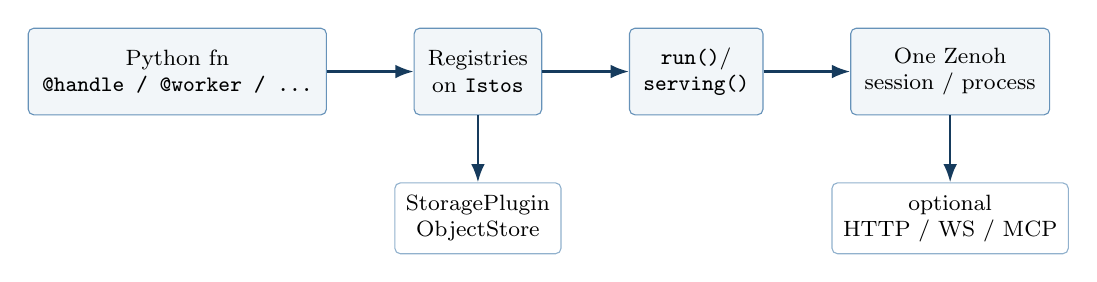
\begin{tikzpicture}[
  font=\footnotesize,
  box/.style={draw=istosblue!70, fill=istosblue!6, rounded corners=2pt,
              align=center, inner sep=5pt, minimum height=1.1cm},
  edge/.style={draw=istosblue!50, rounded corners=2pt, align=center,
               inner sep=4pt, minimum height=0.9cm},
  arr/.style={-{Latex}, thick, istosblue!60!black},
  every node/.style={align=center}
]
\node[box] (py) {Python fn\\{\ttfamily @handle / @worker / \ldots}};
\node[box, right=1.1 of py] (reg) {Registries\\on \texttt{Istos}};
\node[box, right=1.1 of reg] (life) {\texttt{run()}/\\{\ttfamily serving()}};
\node[box, right=1.1 of life] (zen) {One Zenoh\\session / process};
\node[edge, below=0.85 of zen] (edge) {optional\\HTTP / WS / MCP};
\node[edge, below=0.85 of reg] (store) {StoragePlugin\\ObjectStore};
\draw[arr] (py) -- (reg);
\draw[arr] (reg) -- (life);
\draw[arr] (life) -- (zen);
\draw[arr] (zen) -- (edge);
\draw[arr] (reg) -- (store);
\end{tikzpicture}
\end{center}

%==============================================================================
\section{What Istos is (and is not)}
%==============================================================================

Istos is a \textbf{decorator-first Python framework} for distributed services and
multi-agent applications on \textbf{Eclipse Zenoh}. One \texttt{Istos} application
object maps network patterns onto ordinary Python functions.

\paragraph{Product thesis.} Messaging stays explicit as arrows between services;
short TTM (\texttt{pip install}, decorate, \texttt{run()}); same mental model from
laptop to fleet; agent-friendly (channels, leased jobs, HTTP/MCP edge).

\begin{okbox}[Istos is]
\begin{itemize}[leftmargin=*,itemsep=1pt]
  \item A Zenoh-native fabric with FastAPI-like DX (decorators, DI, middleware,
        validation, exception handlers).
  \item Brokerless by default (peer mesh or client$\to$router).
  \item Polyglot on the wire: documented JSON + attachments; no proprietary runtime
        for foreign peers.
\end{itemize}
\end{okbox}

\begin{warnbox}[Istos is not]
\begin{itemize}[leftmargin=*,itemsep=1pt]
  \item A DAG workflow product --- workflows are queue \texttt{chain}/\texttt{group}/\texttt{chord}.
  \item A primary HTTP framework --- HTTP is an optional edge.
  \item ``Celery renamed'' --- control plane is Zenoh queryables; HA is liveliness
        + shared storage, not a broker cluster.
\end{itemize}
\end{warnbox}

\paragraph{Mental model vs FastAPI / Celery.}
\begin{center}
\begin{tabularx}{\textwidth}{@{}lXXX@{}}
\toprule
 & \textbf{FastAPI} & \textbf{Celery} & \textbf{Istos} \\
\midrule
Unit of work & HTTP route & Task & Key-expression endpoint \\
Transport & HTTP & Broker AMQP/Redis & Zenoh \\
Sync request/reply & Natural & Awkward & \texttt{@handle} \\
Background job & BackgroundTasks (weak) & Natural & \texttt{@worker} \\
Streaming & StreamingResponse & N/A & \texttt{@stream} \\
Duplex agent & WebSocket DIY & N/A & \texttt{@channel} \\
Discovery & OpenAPI & Inspect workers & Capabilities + AsyncAPI \\
\bottomrule
\end{tabularx}
\end{center}

%==============================================================================
\section{Architecture and process model}
%==============================================================================

\subsection{Composition}

\texttt{Istos} is mixin-composed over \texttt{IstosBase}
(\texttt{src/istos/app/}):

\begin{center}
\large\texttt{Istos = Messaging + Streaming + Queue + Web + Lifecycle}
\end{center}

\begin{tabularx}{\textwidth}{@{}lX@{}}
\toprule
\textbf{Mixin} & \textbf{Owns} \\
\midrule
Messaging & \texttt{@handle}/\texttt{@query}, pub/sub, liveliness, capabilities \\
Streaming & \texttt{@stream}, channels, \texttt{open\_channel} \\
Queue & owner, workers, enqueue, workflows, schedule \\
Web & HTTP gateway, SSE, WS, MCP, docs UI \\
Lifecycle & \texttt{run}/\texttt{run\_async}/\texttt{serving}, bind/unbind, signals \\
\bottomrule
\end{tabularx}

\subsection{Startup and shutdown}

\paragraph{Bind order} (\texttt{\_LifecycleMixin.\_startup}):
\begin{enumerate}[leftmargin=*,itemsep=1pt]
  \item Logging + built-in handlers (\texttt{.istos/*}).
  \item User \texttt{lifespan} context.
  \item Storage / DB dispose callbacks.
  \item Open Zenoh session (\textbf{one per process}).
  \item Bind: handlers $\to$ streams $\to$ channels $\to$ persist $\to$ queues
        $\to$ publishers $\to$ subscribers $\to$ liveliness.
  \item \texttt{health.ready = True}; optional HTTP server.
\end{enumerate}

Queues bind owners first, then workers, then schedule tasks. Shutdown reverses
unbind; stream queryables share the handler list --- \texttt{\_unbind\_handlers}
tears both down.

\subsection{Async model}

\begin{itemize}[leftmargin=*]
  \item Asyncio-first; sync handlers via \texttt{asyncio.to\_thread}.
  \item Default session: \texttt{AsyncZenohSession}; optional sync via config.
  \item \texttt{@query} / \texttt{publish\_once} \textbf{before} session open
        $\Rightarrow$ \texttt{RuntimeError} (no transient per-call session).
\end{itemize}

\begin{lstlisting}
from contextlib import asynccontextmanager
from istos import Istos

istos = Istos()

@asynccontextmanager
async def on_start(app):
    # Session is open here — safe to query / publish.
    reply = await app.query_once("robot/move", distance=1)
    yield

istos = Istos(lifespan=on_start)
\end{lstlisting}

\subsection{Package map}

\begin{tabularx}{\textwidth}{@{}lX@{}}
\toprule
\textbf{Package} & \textbf{Role} \\
\midrule
\texttt{app/} & Composed API, registries, lifecycle \\
\texttt{primitives/} & Decorator wrappers \\
\texttt{communication/} & Sessions, config, durable, persist \\
\texttt{queue/} & \texttt{QueueRole}, store, workers, cron \\
\texttt{consistency/} & \texttt{StoragePlugin} backends \\
\texttt{http/} & Gateway helpers, ASGI, health, MCP \\
\texttt{security/}, \texttt{di/}, \texttt{middleware/}, \texttt{messages/} & Cross-cutting \\
\texttt{discovery/}, \texttt{observability/} & Capabilities, AsyncAPI, metrics, OTel \\
\texttt{testing/}, \texttt{fitness.py}, \texttt{cli.py} & Tests, architecture fitness, CLI \\
\bottomrule
\end{tabularx}

%==============================================================================
\section{Public API surface}
%==============================================================================

\subsection{Top-level exports}

App: \texttt{Istos}, \texttt{IstosRouter}, \texttt{IstosTestClient}.

Errors: \texttt{IstosError}, \texttt{NotFoundError}, \texttt{UnauthorizedError},
\texttt{ForbiddenError}, \texttt{RateLimitError}, \texttt{ErrorResponse},
\texttt{ERROR\_MARKER}, \texttt{is\_error\_payload}, \texttt{error\_from\_payload},
\texttt{reply\_err}, \texttt{is\_retryable}, \texttt{exception\_handler},
\texttt{IstosSecurityWarning}, \texttt{IstosSecurityError}.

Auth: \texttt{Authorizer}, \texttt{AuthContext}, \texttt{Principal},
\texttt{TokenAuthorizer}, \texttt{JWTAuthorizer}, \texttt{require\_roles}, \texttt{Public}.

Persist / channels / queues: \texttt{ObjectStore}, \texttt{InMemoryObjectStore},
\texttt{S3ObjectStore}, \texttt{PersistRole}, \texttt{ReplayEvent},
\texttt{ChannelSession}, \texttt{ChannelClosed}, \texttt{ChannelClient},
\texttt{SessionStore}, \texttt{QueueStore}, \texttt{QueueRole}, \texttt{JobState},
\texttt{JobRecord}, \texttt{JobContext}.

Other: \texttt{MCPServer}, \texttt{Depends}, \texttt{DependencyCycleError},
\texttt{current\_principal}, \texttt{current\_request}, \texttt{current\_token},
logging helpers.

\subsection{Constructor}

\begin{lstlisting}
Istos(
  session_manager=None,          # XOR with config=
  storage=None,                  # XOR storage_config / storage_database
  lifespan=None,
  config=None,                   # IstosZenohConfig | zenoh.Config
  log_level="INFO", json_logs=False,
  enable_health=True, enable_metrics=True, enable_discovery=True,
  enable_tracing=False, tracing_endpoint=None,
  service_name="istos",          # capabilities key chunk
  exception_registry=None,
  authorizer=None, require_auth=False,  # True + no authorizer -> IstosSecurityError
  http_port=None, enable_mcp=False, mcp_path="/mcp",
)
\end{lstlisting}

\subsection{Decorator catalog with signatures that matter}

\begin{lstlisting}
@app.handle(prefix, serializer=None, retry=None,
            durability="at_most_once", authorizer=None, http=None)
@app.query(key)                          # decorator client
await app.query_once(key, timeout_s=5, serializer=None, token=None,
                     consolidate_replies=True, **params)

@app.stream(...); await app.stream_query(...); @app.stream_client(...)
@app.channel(..., ws=None, durable=False); await app.open_channel(...)
@app.publish(...); @app.subscribe(...); await app.publish_once(...)
app.persist(...); async for ev in app.replay(prefix, since=...)

app.queue(prefix, lease_s=30, max_attempts=5, ha=False, ...)
@app.worker(prefix)
await app.enqueue(prefix, data, delay_s=0, priority=0, token=None)
app.chain(...); app.group(...); app.chord(...)
app.schedule(prefix, data, every_s=... | cron=...)

app.on_liveliness(...); app.declare_liveliness(...)
app.add_middleware(...); app.include_router(...); app.db_session(...)
app.run(); await app.run_async(); async with app.serving(): ...
\end{lstlisting}

\texttt{IstosRouter} records deferred \texttt{action(app)} closures until
\texttt{include\_router}.

%==============================================================================
\section{Worked examples by pattern}
%==============================================================================

\subsection{RPC --- handler + query with lifespan}

\begin{lstlisting}
from contextlib import asynccontextmanager
from istos import Istos, NotFoundError

app = Istos(service_name="fleet")

@app.handle("robot/move", http="POST /move")
async def move(distance: int, speed: str = "normal"):
    if distance < 0:
        raise NotFoundError("no such pose")   # becomes error envelope
    return {"ok": True, "distance": distance, "speed": speed}

@asynccontextmanager
async def boot(app):
    print(await app.query_once("robot/move", distance=10, speed="fast"))
    yield

app = Istos(service_name="fleet", lifespan=boot)
# Wire: get robot/move?distance=10;speed=fast
\end{lstlisting}

\subsection{Stream --- token chunks}

\begin{lstlisting}
@app.stream("llm/generate", http="/llm/generate")  # SSE on gateway
async def generate(prompt: str):
    for token in ("Hello", ", ", "world"):
        yield {"token": token}

async for chunk in app.stream_query("llm/generate", prompt="hi"):
    print(chunk["token"], end="")
# Foreign clients: get with consolidation=None, iterate replies.
\end{lstlisting}

\subsection{Channel --- fabric duplex}

\begin{lstlisting}
from istos import ChannelSession

@app.channel("agent/chat", durable=True, ws="/ws/chat")
async def chat(session: ChannelSession):
    async for msg in session:
        await session.send({"echo": msg})

# Client (after run):
async with await app.open_channel("agent/chat",
                                  conversation_id="conv-1") as ch:
    await ch.send({"text": "hi"})
    print(await ch.receive())
\end{lstlisting}

\paragraph{Fabric handshake (senior detail).}
Client picks session id \(S\); subscribes to \texttt{\{P\}/\{S\}/down}; declares
liveliness at \texttt{\{P\}/\{S\}}; then \texttt{get \{P\}/\{S\}/open}. Server
replies \texttt{\{"ok":true,"sid":"\ldots"\}}. Messages on \texttt{up}/\texttt{down}.
Drop liveliness $\Rightarrow$ peer closes.

\subsection{Pub/sub and queues (preview)}

Full courses: Section~\ref{sec:durability} (all durability layers) and
Section~\ref{sec:queues} (owner, leases, HA, workflows). Quick taste:

\begin{lstlisting}
@app.publish("orders/created", durable=True, cache=1000)
@app.subscribe("orders/created", durable=True, replay=1000)

app.queue("jobs/email", lease_s=30, max_attempts=5)
@app.worker("jobs/email")
async def send(job): ...
await app.enqueue("jobs/email", {"to": "a@b.c", "body": "hi"})
\end{lstlisting}

%==============================================================================
\section{Wire protocol (polyglot)}
\label{sec:wire}
%==============================================================================

Normative: \texttt{docs/reference/wire-protocol.md}. Nothing proprietary beyond
conventions --- Rust/C++/TS Zenoh clients can call and be called.

\subsection{Key expressions}

Decorator \texttt{prefix} \textbf{is} the key. \texttt{*} = one chunk,
\texttt{**} = zero or more.

\begin{center}
\begin{tabular}{@{}ll@{}}
\toprule
Reserved key & Meaning \\
\midrule
\texttt{.istos/health} & liveness \\
\texttt{.istos/ready} & readiness \\
\texttt{.istos/metrics} & metrics snapshot \\
\texttt{.istos/capabilities/<service>} & per-service manifest (fleet-safe) \\
\texttt{.istos/capabilities} & shared --- one arbitrary node answers \\
\texttt{.istos/docs} & AsyncAPI when enabled \\
\bottomrule
\end{tabular}
\end{center}

\subsection{RPC on the wire}

\begin{lstlisting}[language={}]
GET  robot/move?distance=5;speed=fast     # ';' not '&'
ATT  Bearer-or-bare-token | {"tok":"...","cid":"...","tp":"..."}
REP  JSON bytes of return value  OR  error envelope (still JSON)
\end{lstlisting}

Streaming: multi-reply; consumer must disable consolidation or same-key chunks
collapse.

\subsection{Foreign handler checklist}

\begin{enumerate}[leftmargin=*]
  \item Declare queryable on the key.
  \item Parse \texttt{;}-separated selector params.
  \item Authorize from attachment if gated.
  \item Reply serialized result \textbf{or} stamped error envelope.
\end{enumerate}

%==============================================================================
\section{Attachment envelope, correlation, tracing}
\label{sec:envelope}
%==============================================================================

Implementation: \texttt{src/istos/context.py}.

\subsection{Encoding truth table}

\begin{center}
\begin{tabularx}{\textwidth}{@{}lllX@{}}
\toprule
\texttt{tok} & \texttt{cid}/\texttt{tp} & On the wire & Notes \\
\midrule
set & absent & bare UTF-8 string & Compat with old clients \\
set/absent & present & compact JSON object & Short keys only \\
absent & absent & no attachment & Open endpoints \\
\bottomrule
\end{tabularx}
\end{center}

\begin{lstlisting}[language={}]
{"tok":"<token>","cid":"<uuid>","tp":"00-<trace>-<span>-01"}
\end{lstlisting}

\paragraph{Parse rule.} JSON object containing at least one of
\texttt{tok}/\texttt{cid}/\texttt{tp} $\Rightarrow$ envelope; else bare token.
JWTs are never mistaken for envelopes.

\subsection{Correlation ID lifecycle}

\begin{center}
\begin{tikzpicture}[
  font=\scriptsize,
  node distance=0.55cm and 0.7cm,
  step/.style={draw, rounded corners=2pt, fill=gray!8, align=center,
               inner sep=4pt, text width=2.6cm},
  arr/.style={-{Latex}, thick, black!55}
]
\node[step] (http) {HTTP\\X-Correlation-ID\\or mint UUID};
\node[step, right=of http] (att) {Attachment\\{\ttfamily cid}};
\node[step, right=of att] (h1) {Service A\\adopts into\\RequestContext};
\node[step, below=of h1] (h2) {Outbound query\\re-emits cid};
\node[step, left=of h2] (h3) {Service B\\same cid in logs\\+ error envelope};
\draw[arr] (http) -- (att);
\draw[arr] (att) -- (h1);
\draw[arr] (h1) -- (h2);
\draw[arr] (h2) -- (h3);
\end{tikzpicture}
\end{center}

\begin{itemize}[leftmargin=*]
  \item Default mint: \texttt{str(uuid.uuid4())} on \texttt{RequestContext}.
  \item Outbound helpers use \texttt{peek\_request\_context()} --- root calls
        carry \textbf{no} cid/tp (do not invent ambient context).
  \item Errors copy \texttt{correlation\_id} into the envelope; callers recover
        it on \texttt{IstosError} after \texttt{error\_from\_payload}.
\end{itemize}

\subsection{HTTP $\to$ Zenoh mapping}

\begin{center}
\begin{tabular}{@{}ll@{}}
\toprule
HTTP & Attachment / envelope \\
\midrule
\texttt{Authorization: Bearer \ldots} & \texttt{tok} (scheme stripped) \\
\texttt{X-Correlation-ID} or \texttt{X-Request-ID} & \texttt{cid} \\
\texttt{traceparent} & \texttt{tp} \\
\bottomrule
\end{tabular}
\end{center}

\subsection{DI accessors}

\begin{lstlisting}
from istos import Depends, current_request, current_principal, current_token

@app.handle("orders/get")
async def get_order(id: str,
                    req=Depends(current_request),
                    who=Depends(current_principal),
                    tok=Depends(current_token)):
    log.info("cid=%s principal=%s", req.correlation_id, who)
    ...
\end{lstlisting}

%==============================================================================
\section{Errors --- deep dive}
\label{sec:errors}
%==============================================================================

\subsection{Why in-band?}

Polyglot differentiator: foreign peers must not depend on Zenoh
\texttt{reply\_err()} or attachment flags. One JSON object remains the contract.
Unreleased work adds \texttt{\_\_istos\_error} so detection is not a three-key
shape guess.

\subsection{Envelope}

\begin{lstlisting}[language={}]
{
  "__istos_error": true,
  "error": "unauthorized",
  "code": "unauthorized",
  "message": "Not authorized for 'robot/move'",
  "correlation_id": "a1b2-...",
  "details": null
}
\end{lstlisting}

\texttt{ErrorResponse.to\_dict()} always stamps the marker.
\texttt{reply\_err("boom", code="internal\_error")} builds a stamped dict for
\texttt{return} without raising.

\subsection{Detection decision tree}

\begin{lstlisting}[language={}]
is_error_payload(obj):
  if not dict:                         return False
  if "__istos_error" in obj:           return bool(obj["__istos_error"])
  # legacy / foreign peers:
  return "error" in obj and "code" in obj and "message" in obj
\end{lstlisting}

\begin{okbox}[Escape hatch]
Success that legitimately contains \texttt{error}/\texttt{code}/\texttt{message}:
stamp \texttt{"\_\_istos\_error": false}. Prefer redesigning field names when you can.
\end{okbox}

\subsection{Code map}

\begin{center}
\begin{tabular}{@{}llll@{}}
\toprule
\texttt{code} & HTTP & Exception & Retry? \\
\midrule
\texttt{unauthorized} & 401 & \texttt{UnauthorizedError} & no \\
\texttt{forbidden} & 403 & \texttt{ForbiddenError} & no \\
\texttt{not\_found} & 404 & \texttt{NotFoundError} & no \\
\texttt{validation\_error} & 400 & \texttt{IstosError} & no \\
\texttt{bad\_request} & 400 & \texttt{IstosError} & no \\
\texttt{rate\_limit\_exceeded} & 429 & \texttt{RateLimitError} & \textbf{yes} \\
other / \texttt{internal\_error} & 500 & \texttt{IstosError} & yes \\
\bottomrule
\end{tabular}
\end{center}

Status is \textbf{not} on the wire; rebuilt via \texttt{CODE\_TO\_STATUS} for
\texttt{is\_retryable}.

\subsection{Client behaviour}

\begin{itemize}[leftmargin=*]
  \item Single reply: \texttt{query\_once} / \texttt{@query} / streams / channels /
        queue control \textbf{raise} \texttt{error\_from\_payload(...)}.
  \item Multi-reply list: returned as data; filter with
        \texttt{is\_error\_payload} per item.
  \item Empty / timeout: \texttt{[]} --- \textbf{not} an exception; retries do not fire.
  \item Handler \texttt{return None}: no Zenoh reply $\Rightarrow$ same empty path.
\end{itemize}

\begin{lstlisting}
from istos import is_error_payload, error_from_payload, NotFoundError

try:
    return await app.query_once("clients/get", id="acme")
except NotFoundError:
    return None

replies = await app.query_once("*/health", consolidate_replies=False)
alive = [r for r in replies if not is_error_payload(r)]
\end{lstlisting}

\subsection{Producers (must stamp)}

Handlers (exception registry), streams, queue refusals, fabric channel
open/auth, HTTP gateway local errors --- all via \texttt{to\_dict()} /
\texttt{reply\_err}. Do not hand-build partial error dicts.

\subsection{\texttt{is\_retryable}}

\begin{lstlisting}
def is_retryable(exc):
    if isinstance(exc, IstosError):
        if exc.status == 429: return True
        return not (400 <= exc.status < 500)
    return True  # TimeoutError, transport, ...
\end{lstlisting}

%==============================================================================
\section{Security}
%==============================================================================

\subsection{Default = open}

Peer + multicast + no authorizer. Local demos are easy; production copy-paste is
dangerous. \texttt{IstosSecurityWarning} on insecure open --- escalate in CI.

\begin{lstlisting}
import warnings
from istos import IstosSecurityWarning
warnings.simplefilter("error", IstosSecurityWarning)
\end{lstlisting}

\subsection{Two layers you must both do}

\begin{enumerate}[leftmargin=*]
  \item \textbf{Transport:} TLS/mTLS, credentials, \texttt{mode="client"},
        \texttt{multicast\_scouting=False}.
  \item \textbf{App:} \texttt{authorizer=} + prefer \texttt{require\_auth=True}.
\end{enumerate}

\subsection{Authorizers}

\begin{lstlisting}
from istos import Istos, TokenAuthorizer, JWTAuthorizer, require_roles, Public

app = Istos(
  require_auth=True,
  authorizer=JWTAuthorizer(secret=os.environ["JWT_SECRET"], audience="api"),
)

@app.handle("admin/stats", authorizer=require_roles("admin"))
async def stats(): ...

@app.handle("public/ping", authorizer=Public)   # opt out of app gate
async def ping(): return {"ok": True}
\end{lstlisting}

Auth is a \textbf{network-boundary gate before} middleware. HTTP strips
\texttt{Bearer}; pure Zenoh attachments should carry the bare JWT.

\begin{warnbox}[Edge auth $\neq$ fabric auth]
Protecting \texttt{http\_port} does not protect peers that speak Zenoh directly
to your queryables. Secure the fabric itself.
\end{warnbox}

%==============================================================================
\section{Request pipeline (RPC)}
%==============================================================================

\begin{enumerate}[leftmargin=*,itemsep=2pt]
  \item Queryable receives Zenoh query.
  \item Decode selector params; parse attachment $\to$ \texttt{RequestEnvelope}.
  \item Authorizer(\texttt{AuthContext}).
  \item Build \texttt{RequestContext} (adopt \texttt{cid}/\texttt{tp}).
  \item Middleware onion (outer first): CorrelationId $\to$ Logging $\to$
        Prometheus? $\to$ Tracing? $\to$ user middlewares.
  \item DI (\texttt{Depends}, overrides, \texttt{db\_session}).
  \item Durability ledger if not \texttt{at\_most\_once}.
  \item Handler body.
  \item Serialize success --- or registry $\to$ error envelope +
        \texttt{correlation\_id}.
\end{enumerate}

%==============================================================================
\section{DI, validation, middleware}
%==============================================================================

\subsection{Depends}

Sync/async/generators; cycles $\to$ \texttt{DependencyCycleError}.
\texttt{app.dependency\_overrides[fn] = mock}. Injected names skipped in network
validation. Workers get \texttt{Depends} the same way as handlers.

\subsection{Validation}

Annotations / Pydantic at the edge $\to$ \texttt{validation\_error} envelope.

\subsection{Exception handlers}

\begin{lstlisting}
from istos import ErrorResponse

@app.exception_handler(ValueError)
def on_value(exc: ValueError) -> ErrorResponse:
    return ErrorResponse(error="bad_request", code="bad_request",
                         message=str(exc))
\end{lstlisting}

%==============================================================================
\section{Durability --- complete course}
\label{sec:durability}
%==============================================================================

Istos has \textbf{three separate durability stories}. Mixing up their names is the
most common senior mistake. Learn them as different crash domains.

\begin{center}
\begin{tabularx}{\textwidth}{@{}lXXX@{}}
\toprule
 & \textbf{A. Handler ledger} & \textbf{B. Advanced pub/sub} & \textbf{C. Persist role} \\
\midrule
API & \texttt{durability=} on \texttt{@handle} & \texttt{durable=True} & \texttt{persist=} / \texttt{app.persist} \\
Crash domain & Duplicate RPC delivery & Late join / blip & Producer process death \\
Holds data & \texttt{StoragePlugin} & Producer RAM cache & S3 / memory ObjectStore \\
Guarantee & at-most / at-least / exactly & at-least within window & history after producer gone \\
\bottomrule
\end{tabularx}
\end{center}

\begin{keybox}[Jobs are a fourth story]
Work queues write through to the same \texttt{StoragePlugin} as (A), but their
semantics are leases + ack/nack --- see Section~\ref{sec:queues}. Do not call a
queue ``durable pub/sub''.
\end{keybox}

\subsection{A --- Handler durability (\texttt{StoragePlugin})}

Used so RPC side effects are not doubled when a client retries.

\begin{lstlisting}
from istos.consistency import RedisStoragePlugin

app = Istos(storage=RedisStoragePlugin(url="redis://localhost:6379/0",
                                       prefix="istos:"))

@app.handle("payments/charge", durability="exactly_once")
async def charge(payment_id: str, amount: float):
    return {"charged": amount}
\end{lstlisting}

\begin{center}
\begin{tabular}{@{}p{0.22\textwidth}p{0.35\textwidth}p{0.35\textwidth}@{}}
\toprule
Mode & Storage ops & Semantics \\
\midrule
\texttt{at\_most\_once} & best-effort metadata & Default; fastest; may lose ledger \\
\texttt{at\_least\_once} & \texttt{log(...)} & Retries may duplicate side effects \\
\texttt{exactly\_once} & \texttt{check\_processed} $\to$ short-circuit;
  then \texttt{log} + \texttt{mark\_processed} & Same network params $\Rightarrow$
  cached result \\
\bottomrule
\end{tabular}
\end{center}

\paragraph{Idempotency key.}
\texttt{sha256(f"\{prefix\}:\{json.dumps(params, sort\_keys=True, default=str)\}")}
over \textbf{network params only} (DI-injected args excluded).

\paragraph{StoragePlugin protocol.}
\texttt{put}/\texttt{get}/\texttt{delete}, \texttt{log}/\texttt{get\_log},
\texttt{check\_processed}/\texttt{mark\_processed}.

\begin{center}
\begin{tabular}{@{}lll@{}}
\toprule
Backend & Install & Use \\
\midrule
\texttt{InMemoryStoragePlugin} & built-in & Dev/tests; volatile \\
\texttt{RedisStoragePlugin} & \texttt{istos[redis]} & Shared across processes \\
\texttt{SqlAlchemyStoragePlugin} & \texttt{istos[sqlalchemy]} + driver & Postgres/SQLite/\ldots \\
\bottomrule
\end{tabular}
\end{center}

\begin{lstlisting}
# SQLAlchemy example
from istos.consistency import SqlAlchemyStoragePlugin
app = Istos(storage=SqlAlchemyStoragePlugin(
    "postgresql+asyncpg://user:pass@db:5432/istos"))
\end{lstlisting}

Also powers: queue write-through, channel \texttt{SessionStore} history
(\texttt{conv:\{id\}}).

\subsection{B --- Brokerless durable pub/sub (\texttt{durable=True})}

No Kafka. The \textbf{producer} keeps a bounded replay cache and heartbeats a
sequence number. Late / reconnecting subscribers recover \textbf{peer-to-peer}
via Zenoh advanced pub/sub (\texttt{zenoh.ext}).

\begin{lstlisting}
@app.publish("orders/created", durable=True, cache=1000, heartbeat=1.0)
async def created(order: dict):
    return order

@app.subscribe("orders/created", durable=True, replay=1000, recover=True,
               on_miss=lambda src, n: alert(f"lost {n} from {src}"))
async def on_created(event: dict):
    await process(event)   # keep idempotent
\end{lstlisting}

\begin{center}
\begin{tabular}{@{}lll@{}}
\toprule
Side & Option & Meaning \\
\midrule
publish & \texttt{cache} & Samples retained for replay (default 1000) \\
publish & \texttt{heartbeat} & Seq heartbeat seconds (default 1.0) \\
publish & reliability / congestion & Default RELIABLE + BLOCK (no silent drop) \\
subscribe & \texttt{replay} & Max historical samples on join \\
subscribe & \texttt{recover} & Re-fetch gaps after blips \\
subscribe & \texttt{on\_miss} & Unrecoverable gap callback \\
\bottomrule
\end{tabular}
\end{center}

\begin{warnbox}[Honest limits of advanced durable]
Replay is \textbf{bounded by cache}. If the producer restarts, its RAM cache is
gone. That is when you need layer C (\texttt{persist=}), or a Zenoh router
storage plugin (out of band). Cannot combine \texttt{durable=True} with
\texttt{use\_shm=True}.
\end{warnbox}

\paragraph{Guarantees.} At-least-once within the retained window; effectively-once
only with idempotent consumers (+ optional handler ledger for RPC).

\subsection{C --- Persist role (survive producer death)}

\texttt{persist="s3://\ldots"} (or \texttt{memory://}, or an \texttt{ObjectStore})
co-locates a writer + history queryable:

\begin{itemize}[leftmargin=*]
  \item Writer stores \textbf{every} sample under a minted per-sample key
        \texttt{<prefix>/<unix\_millis>-<seq>} (stream, not last-value).
  \item History queryable answers \texttt{get(prefix/**)}.
  \item Foreign languages: wildcard get; do not query the bare key (consolidation).
\end{itemize}

\begin{lstlisting}
# On publisher
@app.publish("orders/created", durable=True, persist="s3://orders-log")
async def created(order: dict): return order

# On subscriber — works even if original producer crashed
@app.subscribe("orders/created", durable=True, replay_persisted=True)
async def on_created(event: dict): await process(event)

# Standalone storage node (no publishers of its own)
app.persist("orders/created", "s3://orders-log")

# Cursor-based batch replay
async for ev in app.replay("orders/created", since=cursor):
    await project(ev.data)
    cursor = ev.position   # opaque; checkpoint yourself
\end{lstlisting}

Needs \texttt{istos[s3]} for S3/MinIO; credentials via AWS chain (not in URL).
Store write failures are logged and swallowed --- they never crash the producer.
Replayed persisted samples skip the authorizer (trusted store); may interleave
with live/cache replay $\Rightarrow$ \textbf{idempotent callbacks}.

\subsection{Durability decision tree}

\begin{lstlisting}[language={}]
Need late join while producer is up?     -> durable=True
Need history after producer dies?        -> persist= / app.persist + replay_persisted
Need RPC not to double-charge?           -> durability="exactly_once" + shared storage
Need one worker, retries, DLQ?           -> work queue (next section), not pub/sub
Need fan-out to everyone?                -> pub/sub (optionally durable/persist)
\end{lstlisting}

\subsection{Channel durability (bonus)}

\texttt{@channel(durable=True)} uses \texttt{SessionStore} over the same
\texttt{StoragePlugin} (\texttt{log}/\texttt{get\_log} under
\texttt{conv:\{conversation\_id\}}). Resume with \texttt{conversation\_id=} on
open / WS. This is conversation history, not pub/sub persist.

%==============================================================================
\section{Work queues --- complete course}
\label{sec:queues}
%==============================================================================

\subsection{Job vs event}

\begin{center}
\begin{tabularx}{\textwidth}{@{}X X@{}}
\toprule
\textbf{Event (pub/sub)} & \textbf{Job (work queue)} \\
\midrule
Every interested party should see it & Exactly one worker should do it \\
``Order was created'' & ``Send this email'' / ``Apply this patch'' \\
Losing a subscriber is often OK & Losing the job is not \\
Optional durable/persist for late join & Leases, ack/nack, backoff, DLQ \\
\bottomrule
\end{tabularx}
\end{center}

\subsection{Owner model (no broker)}

One node is the \textbf{owner}: holds jobs, hands out claims, tracks leases,
dead-letters, sweeps. Workers anywhere claim over Zenoh. Single owner $\Rightarrow$
two workers never hold the same job concurrently.

\begin{lstlisting}[language={}]
        enqueue                 claim / ack / nack
  producer ─────► ┌───────────────┐ ◄───────── worker A
                  │  QUEUE OWNER   │ ◄───────── worker B
                  │  · jobs/leases │  sweeper reclaims expired leases
                  │  · dead-letter │
                  └───────────────┘
                         ▲
                  put {prefix}/notify  (wake idle workers)
\end{lstlisting}

Control queryables under \texttt{\{prefix\}/}: \texttt{enqueue}, \texttt{claim},
\texttt{ack}, \texttt{nack}, \texttt{result}, \texttt{dead}, \texttt{chord}.

\subsection{The three roles --- minimal complete example}

\begin{lstlisting}
from istos import Istos, JobContext

app = Istos()   # add RedisStoragePlugin for durability / HA

# 1. Own
app.queue("jobs/email",
          lease_s=30,
          max_attempts=5,
          sweep_interval_s=5.0,
          retry_backoff_s=1.0,
          retry_backoff_max_s=600.0,
          retry_jitter=0.1,
          keep_results=False,
          result_ttl_s=3600.0,
          ha=False)

# 2. Work — return = ack, raise = nack
@app.worker("jobs/email", concurrency=4)
async def send(job, ctx: JobContext):
    if ctx.is_last_attempt:
        await alert_ops(ctx.job_id, ctx.last_error)
    await smtp.send(job["to"], job["body"])

# 3. Produce
job_id = await app.enqueue("jobs/email",
                           {"to": "a@b.com", "body": "hi"},
                           priority=10, delay_s=0)
\end{lstlisting}

\subsection{Job state machine}

\begin{center}
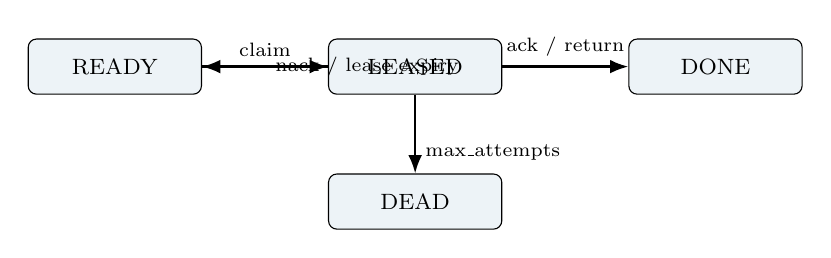
\begin{tikzpicture}[
  font=\footnotesize,
  st/.style={draw, rounded corners=3pt, minimum width=2.2cm, minimum height=0.7cm,
             fill=istosblue!8, align=center},
  arr/.style={-{Latex}, thick}
]
\node[st] (ready) {READY};
\node[st, right=1.6 of ready] (leased) {LEASED};
\node[st, right=1.6 of leased] (done) {DONE};
\node[st, below=1.0 of leased] (dead) {DEAD};
\draw[arr] (ready) -- node[above,font=\scriptsize]{claim} (leased);
\draw[arr] (leased) -- node[above,font=\scriptsize]{ack / return} (done);
\draw[arr] (leased) -- node[right,font=\scriptsize]{nack / lease expiry} (ready);
\draw[arr] (leased) -- node[below right,font=\scriptsize]{max\_attempts} (dead);
\end{tikzpicture}
\end{center}

\paragraph{Leases.} Claim grants \texttt{lease\_s} seconds. Crash without ack/nack
$\Rightarrow$ sweeper returns job to READY. Pick \texttt{lease\_s} slightly above
slowest healthy job. Processing must be \textbf{idempotent}: crash after side
effect but before ack redelivers (at-least-once).

\subsection{Backoff formula}

After attempt $n$ fails (nack), next eligibility waits approximately:
\[
\min\!\bigl(\texttt{retry\_backoff\_s}\cdot 2^{\max(0,n-1)},\;
\texttt{retry\_backoff\_max\_s}\bigr)
\cdot (1 + U[-\texttt{jitter},+\texttt{jitter}])
\]
Stored on the job as \texttt{not\_before}. Default base $1\,\mathrm{s}$, cap
$600\,\mathrm{s}$, jitter $0.1$.

\subsection{\texttt{JobRecord} and \texttt{JobContext}}

\paragraph{JobRecord (owner store):}
\texttt{id}, \texttt{data} (raw body bytes), \texttt{state}, \texttt{attempts},
\texttt{max\_attempts}, \texttt{enqueued\_at}, \texttt{lease\_until},
\texttt{not\_before}, \texttt{priority} (higher first), \texttt{seq} (FIFO
tiebreak), \texttt{last\_error}, \texttt{result} (optional base64),
\texttt{completed\_at}, \texttt{wf} (chain/chord JSON).

\paragraph{JobContext (worker opt-in \texttt{ctx} param):}
\texttt{job\_id}, \texttt{queue}, \texttt{attempt} (1-based), \texttt{max\_attempts},
\texttt{last\_error}, \texttt{is\_retry}, \texttt{is\_last\_attempt}.
\texttt{Depends(...)} still wins if \texttt{ctx} is a dependency.

\subsection{Dead letters}

After \texttt{max\_attempts}, job is DEAD --- never auto-redelivered.

\begin{lstlisting}
for job in await app.dead_letters("jobs/email"):
    log.error("%s failed %s times: %s",
              job["job_id"], job["attempts"], job["last_error"])
    # deliberate re-enqueue after fix — no magic "revive" button
    await app.enqueue("jobs/email", job["data"])
\end{lstlisting}

\subsection{Scaling workers}

\begin{itemize}[leftmargin=*]
  \item \texttt{concurrency=N} --- N claim loops in one process (I/O-bound).
  \item More processes with the same \texttt{@worker} --- competing consumers;
        owner arbitrates.
  \item Hot path: owner \texttt{put \{prefix\}/notify}; \texttt{poll\_interval\_s}
        is a safety net for delays/redelivery, not busy-wait.
\end{itemize}

Hot-path ops are $O(\log n)$ heaps --- deep backlog should not slow the next claim.

\subsection{Delay, priority, results}

\begin{lstlisting}
await app.enqueue("jobs/email", welcome, priority=10)
await app.enqueue("jobs/email", digest, delay_s=3600)

app.queue("jobs/render", keep_results=True, result_ttl_s=3600)
outcome = await app.result("jobs/render", job_id)
# state: ready | leased | done | dead | unknown (aged out)
\end{lstlisting}

\subsection{Schedule (beat)}

\begin{lstlisting}
app.queue("jobs/report")
app.schedule("jobs/report", {"kind": "hourly"}, every_s=3600)
app.schedule("jobs/report", {"kind": "nightly"}, cron="0 2 * * *")
# cron: min hour dom month dow — *, ranges, steps, lists; DOM∪DOW like Vixie
\end{lstlisting}

\begin{warnbox}[Who ticks?]
Co-located with HA owner: fires only when \texttt{QueueRole.is\_active} (leader).\\
Standalone scheduler (no local owner): \textbf{every} such process ticks --- run
exactly one, or you double-enqueue.
\end{warnbox}

\subsection{Workflows: chain, group, chord}

\begin{lstlisting}
# Pipeline: each return feeds the next
await app.chain(["jobs/fetch", "jobs/parse", "jobs/store"], url)

# Parallel batch on one queue
ids = await app.group("jobs/thumbnail", [img1, img2, img3])

# Parallel + barrier callback (results in order + your meta)
await app.chord("jobs/shard", shards,
                callback=("jobs/reduce", {"job": "nightly"}))
# reduce receives {"results": [...], "input": {"job": "nightly"}}
\end{lstlisting}

Continuations enqueue before ack --- crash redelivers the step (keep idempotent).
A dead-lettered chord member \textbf{stalls} the barrier; fix and re-enqueue.

\subsection{Queue durability and HA}

\paragraph{Durability.} Owner memory is authoritative; every mutation write-through
to app \texttt{StoragePlugin}. In-memory $\Rightarrow$ restart loses jobs. Redis /
SQLAlchemy $\Rightarrow$ reload on startup; sweeper cleans mid-flight leases.

\begin{lstlisting}
from istos.consistency import RedisStoragePlugin
app = Istos(storage=RedisStoragePlugin(url="redis://localhost:6379/0"))
app.queue("jobs/email")          # survives owner restart
app.queue("jobs/email", ha=True) # + failover (needs shared storage)
\end{lstlisting}

\paragraph{HA.} \texttt{ha=True}: replicas declare liveliness
\texttt{\{prefix\}/\_owners/\{id\}}; lowest live id leads and binds queryables.
Leader death $\Rightarrow$ token drop $\Rightarrow$ standby activates and recovers
jobs. Election is leaderless-recovery, not consensus --- brief overlap possible
(still at-least-once). Producers/workers unchanged.

\begin{warnbox}[HA + in-memory = false HA]
Without shared storage each replica is an island. Always pair \texttt{ha=True}
with Redis or SQLAlchemy.
\end{warnbox}

\subsection{Queue guarantees (plainly)}

\begin{itemize}[leftmargin=*]
  \item \textbf{At-least-once}, not exactly-once --- idempotent workers.
  \item \textbf{One at a time} --- single active owner serializes claims.
  \item \textbf{Bounded retries} --- then DLQ; cannot spin forever.
  \item \textbf{Owner tracks ack state} --- give it durable storage; use HA for
        failover.
\end{itemize}

\subsection{Jobs vs RPC payloads (again)}

\texttt{@query} puts args in the selector (URL-quoted). Fine for small commands;
wrong for source files / patches. Those are job bodies. The fable-workflow example
is built on this rule.

\subsection{Auth on queues}

\texttt{app.queue(..., authorizer=...)} gates enqueue/claim/result/dead/etc.
Refusals are stamped error envelopes; clients raise (0.2.0+). Workers with bad
tokens log and keep polling.

%==============================================================================
\section{HTTP, ASGI, MCP, discovery}
%==============================================================================

\subsection{Gateway}

With \texttt{http\_port}: \texttt{/livez}, \texttt{/readyz}, \texttt{/metrics},
routes from \texttt{http=}/\texttt{ws=}, optional MCP + AsyncAPI UI.
\texttt{status\_for\_reply} maps error envelopes to HTTP statuses.

\subsection{ASGI}

\texttt{from istos.http.asgi import lifespan} --- co-host fabric inside FastAPI;
ASGI owns HTTP, Istos owns Zenoh.

\subsection{MCP}

\texttt{enable\_mcp=True}: tools from \texttt{@handle} (skip \texttt{.istos/*});
names \texttt{prefix.replace("/", "-")}; \texttt{tools/call} $\to$
\texttt{query\_once}.

\subsection{Capabilities discovery}

\begin{lstlisting}
# Wrong mental model: bare key fans out to the fleet — it does NOT.
manifest = await app.query_once(".istos/capabilities")  # one node

# Right: per-service keys + consolidation off
fleet = await app.discover_capabilities()
# = get .istos/capabilities/* with consolidate_replies=False
\end{lstlisting}

Service name sanitized: non-\texttt{[A-Za-z0-9\_.-]} $\to$ \texttt{-}. Replicas
sharing a name share a key (by design).

%==============================================================================
\section{Configuration}
%==============================================================================

\texttt{IstosZenohConfig} --- env prefix \texttt{ISTOS\_ZENOH\_},
\texttt{extra="forbid"}:

\begin{lstlisting}[language={}]
ISTOS_ZENOH_MODE=client
ISTOS_ZENOH_CONNECT_ENDPOINTS=["tls/zenoh-router.local:7447"]
ISTOS_ZENOH_MULTICAST_SCOUTING=false
ISTOS_ZENOH_USERNAME=svc
ISTOS_ZENOH_PASSWORD=...
ISTOS_ZENOH_ROOT_CA_CERTIFICATE=/path/ca.pem
# mTLS: LISTEN_CERTIFICATE + LISTEN_PRIVATE_KEY + ENABLE_MTLS=true
\end{lstlisting}

Raw PEM strings accepted for secret managers. Warns if no TLS/auth, or auth
without TLS.

%==============================================================================
\section{Testing, fitness, CLI}
%==============================================================================

\paragraph{\texttt{IstosTestClient}.} In-process: authorizer, validation, DI,
durability --- \textbf{no Zenoh}. Use for unit/contract tests; mark live mesh
tests \texttt{@pytest.mark.integration}.

\paragraph{CLI.} \texttt{istos new}, \texttt{istos analyze} (abstractness /
instability / distance, cycles), \texttt{istos docs}, \texttt{istos version}.

%==============================================================================
\section{Case study --- fable-workflow}
%==============================================================================

\texttt{examples/fable-workflow} turns the Fable Method into \textbf{structure}
instead of prompt hope:

\begin{itemize}[leftmargin=*]
  \item Four processes: orchestrator, evidence lenses, executor, judge.
  \item Evidence in parallel via queues (not RPC --- bodies are large).
  \item Executor cannot mark success: judge (separate process, no shared FS)
        ack/nacks.
  \item \texttt{max\_attempts=3} is the stop condition (DLQ), not model manners.
\end{itemize}

\begin{keybox}[Lesson for agent systems]
If a property matters, encode it in process boundaries and queue semantics, not
in instructions the same model can ignore.
\end{keybox}

%==============================================================================
\section{Debugging cookbook}
%==============================================================================

\begin{tabularx}{\textwidth}{@{}>{\raggedright\arraybackslash}p{0.34\textwidth}X@{}}
\toprule
\textbf{Symptom} & \textbf{Check} \\
\midrule
\texttt{[]} from \texttt{query\_once} & Handler returned \texttt{None}? Wrong key?
Timeout? No responder (complete routing)? \\
Outage looks like empty list & Pre-0.2 client treating error dict as data?
Upgrade / raise on envelope. \\
Success raises as error & Body has error+code+message without
\texttt{\_\_istos\_error:false}? Legacy peer? \\
Only one node answers fleet query & Same key + \texttt{complete=True}. Use distinct
keys + \texttt{consolidate\_replies=False}. \\
HA queue loses jobs & In-memory storage? Need Redis/SQL. \\
Late join got nothing & Producer down + no \texttt{persist}? Cache-only durable. \\
Duplicate charges on retry & Missing \texttt{exactly\_once} or non-idempotent worker. \\
Chord never finishes & Member in DLQ --- inspect \texttt{dead\_letters}. \\
Double cron fires & Multiple \texttt{schedule} nodes without local owner gate. \\
JWT fails on fabric, works on HTTP & \texttt{Bearer } still in attachment? Strip. \\
cid missing in service B & A didn't run inside a request context, or foreign
client omitted \texttt{cid}. \\
Stream hangs after last chunk & Old bug; ensure stream closes query (fixed 0.1.2+). \\
SSE idle 60s & Same --- stream finalize / timeout. \\
\bottomrule
\end{tabularx}

\paragraph{Log correlation.}
Always log \texttt{RequestContext.correlation\_id}. On failure, the envelope's
\texttt{correlation\_id} should match the responder's line.

%==============================================================================
\section{Footguns}
\label{sec:footguns}
%==============================================================================

\begin{enumerate}[leftmargin=*,itemsep=3pt]
  \item \textbf{\texttt{complete=True}} --- same key is not fan-out.
  \item \textbf{Open fabric defaults} --- secure transport + \texttt{require\_auth}.
  \item \textbf{HA needs shared storage}.
  \item \textbf{Multi-reply} --- check each envelope yourself.
  \item \textbf{\texttt{None} = no reply} $\neq$ exception.
  \item \textbf{Timeout $\neq$ retryable exception}.
  \item \textbf{Error-shaped success} --- marker \texttt{false} or rename fields.
  \item \textbf{Serializer mismatch} between peers.
  \item \textbf{JWT Bearer on Zenoh} --- HTTP strips; fabric may not.
  \item \textbf{Schedule topology} --- one beat source.
  \item \textbf{Chord + DLQ} can stall.
  \item \textbf{RPC selectors vs job bodies} for large payloads.
  \item \textbf{Legacy three-key fallback} with old foreign peers.
  \item \textbf{Capabilities bare key} is not fleet discovery.
\end{enumerate}

%==============================================================================
\section{Anti-patterns vs patterns}
%==============================================================================

\begin{center}
\begin{tabularx}{\textwidth}{@{}X X@{}}
\toprule
\textbf{Anti-pattern} & \textbf{Pattern} \\
\midrule
Put a file in selector params & Enqueue job with body \\
N identical \texttt{@handle("health")} for fleet & \texttt{\{name\}/health} + wildcard get \\
\texttt{if reply.get("code")} after 0.2 & \texttt{except NotFoundError} \\
In-memory + \texttt{ha=True} in prod & Redis/SQLAlchemy storage \\
\texttt{durable=True} expecting crash survival & Add \texttt{persist=} / standalone role \\
Pub/sub for ``send email once'' & Work queue + idempotent worker \\
Non-idempotent worker + short lease & Idempotent side effects; tune \texttt{lease\_s} \\
Auth only on HTTP gateway & Fabric TLS + app authorizer \\
One mega-process for judge+executor & Separate processes / trust boundaries \\
Ignore \texttt{cid} in foreign client & Always forward envelope metadata \\
Custom error dict missing fields & \texttt{raise IstosError} or \texttt{reply\_err} \\
\bottomrule
\end{tabularx}
\end{center}

%==============================================================================
\section{Production topology sketches}
%==============================================================================

\paragraph{Laptop demo.} Peer mode, multicast, in-memory storage, no auth --- fine
inside \texttt{IstosSecurityWarning}.

\paragraph{Single router prod.}
\begin{lstlisting}[language={}]
services --client+TLS--> zenoh-router <--client+TLS-- workers
storage: Redis/Postgres shared by queue owners (ha=True)
one schedule beat (or co-locate with HA owner)
HTTP edge pods: gateway only; fabric still authenticated
\end{lstlisting}

\paragraph{Agent mesh.} Orchestrator owns queues; evidence/executor/judge are
workers; judge cannot see executor FS; DLQ is the human escalation path.

%==============================================================================
\section{Operational checklist}
%==============================================================================

\begin{itemize}[leftmargin=*]
  \item[$\square$] TLS/mTLS; multicast off in shared networks
  \item[$\square$] \texttt{require\_auth=True}; review every \texttt{Public}
  \item[$\square$] Shared storage for HA queues
  \item[$\square$] Distinct \texttt{service\_name}; discover with consolidation off
  \item[$\square$] Foreign clients forward \texttt{cid}/\texttt{tp}
  \item[$\square$] Alert/search logs by \texttt{correlation\_id}
  \item[$\square$] \texttt{/readyz} + \texttt{.istos/ready}; scrape \texttt{/metrics}
  \item[$\square$] CI: \texttt{IstosSecurityWarning} as error
  \item[$\square$] Integration tests marked and run in CI
  \item[$\square$] Serializer pairs documented per endpoint
\end{itemize}

%==============================================================================
\section{PR review checklist (Istos-specific)}
%==============================================================================

\begin{itemize}[leftmargin=*]
  \item[$\square$] Right primitive? (RPC vs stream vs channel vs queue vs pub/sub)
  \item[$\square$] Key design: collisions / \texttt{complete=True} implications?
  \item[$\square$] Large payloads on jobs, not selectors?
  \item[$\square$] Durability layer chosen consciously?
        (handler ledger vs \texttt{durable=} vs \texttt{persist=} vs queue store)
  \item[$\square$] Workers / subscribers idempotent where at-least-once applies?
  \item[$\square$] Queue: \texttt{lease\_s}, \texttt{max\_attempts}, storage, HA coherent?
  \item[$\square$] Schedule topology: one beat source?
  \item[$\square$] Errors via raise / \texttt{reply\_err}, not ad-hoc dicts?
  \item[$\square$] Authz on new endpoints; \texttt{Public} justified?
  \item[$\square$] Outbound calls inherit cid; foreign hops documented?
  \item[$\square$] Tests: TestClient for logic; integration for mesh / leases?
  \item[$\square$] Capabilities / AsyncAPI updated if surface changed?
\end{itemize}

%==============================================================================
\section{Version awareness}
%==============================================================================

\begin{itemize}[leftmargin=*]
  \item \textbf{0.2.0} --- raise on error envelopes; per-service capabilities;
        smarter retry; standardized queue refusal envelopes.
  \item \textbf{Unreleased} --- \texttt{\_\_istos\_error} + \texttt{reply\_err};
        HA-aware schedule; SECURITY.md / architecture diagram sync.
\end{itemize}

Read \texttt{docs/changelog.md} before upgrading. Wire-protocol.md is normative
for polyglot work.

%==============================================================================
\section{Glossary}
%==============================================================================

\begin{description}[style=nextline,leftmargin=2.4cm,font=\ttfamily\footnotesize]
  \item[key expression] Zenoh address; Istos \texttt{prefix}.
  \item[queryable] Server-side RPC/stream endpoint.
  \item[complete] Queryable flag: this responder fully answers the key.
  \item[attachment] Out-of-band bytes: bare token or envelope.
  \item[envelope] JSON \texttt{tok}/\texttt{cid}/\texttt{tp} in attachment.
  \item[cid] Correlation id spanning hops.
  \item[tp] W3C \texttt{traceparent}.
  \item[ERROR\_MARKER] \texttt{\_\_istos\_error} discriminator.
  \item[StoragePlugin] App ledger: KV, event log, idempotency.
  \item[handler durability] \texttt{at\_most\_once}/\texttt{at\_least\_once}/\texttt{exactly\_once}.
  \item[durable=] Advanced Zenoh pub/sub replay cache (producer RAM).
  \item[persist=] Object-store stream history (survives producer death).
  \item[PersistRole] Writer + history queryable for a key.
  \item[ReplayEvent] \texttt{position}, \texttt{data}, \texttt{timestamp\_ms}.
  \item[QueueRole] Owner process for a work queue.
  \item[JobRecord] Authoritative job row in the owner store.
  \item[JobContext] Per-delivery metadata injected as \texttt{ctx}.
  \item[lease] Time budget for a claimed job before redelivery.
  \item[dead letter] Job that exhausted \texttt{max\_attempts}.
  \item[notify] Owner put that wakes idle workers.
  \item[chain/group/chord] Sequential / parallel / barrier workflows.
  \item[liveliness] Zenoh presence (HA election, channel presence).
  \item[SessionStore] Durable channel conversation log via storage.
\end{description}

%==============================================================================
\section{Source map}
%==============================================================================

\begin{tabularx}{\textwidth}{@{}lX@{}}
\toprule
\textbf{Topic} & \textbf{Path} \\
\midrule
Exports / constructor & \texttt{src/istos/\_\_init\_\_.py}, \texttt{app/\_base.py} \\
Envelope / context & \texttt{src/istos/context.py} \\
Errors & \texttt{src/istos/errors.py} \\
Auth & \texttt{src/istos/security/authz.py} \\
Handler path & \texttt{src/istos/primitives/handler.py} \\
Wire contract & \texttt{docs/reference/wire-protocol.md} \\
RPC / security guides & \texttt{docs/user-guide/rpc.md}, \texttt{security.md} \\
\textbf{Durability guides} & \texttt{durable-messaging.md}, \texttt{storage.md} \\
\textbf{Queue guide} & \texttt{docs/user-guide/work-queues.md} \\
Queue code & \texttt{app/queues.py}, \texttt{queue/role.py}, \texttt{queue/store.py} \\
Persist code & \texttt{communication/persist.py} \\
Channels & \texttt{primitives/channel\_fabric.py}, \texttt{session\_store.py} \\
Config & \texttt{communication/config.py} \\
Lifecycle & \texttt{app/lifecycle.py} \\
Gateway & \texttt{http/gateway.py}, \texttt{app/web.py} \\
Example system & \texttt{examples/fable-workflow/} \\
Architecture sketch & \texttt{istos\_architecture.puml} \\
\bottomrule
\end{tabularx}

\vspace{1.2em}
\begin{center}
\begin{tcolorbox}[colback=istosblue!5, colframe=istosblue!60, width=0.95\textwidth]
\centering
\textbf{Closing rule.}\\[0.35em]
Design with keys and primitives first, then auth, then the \emph{right}
durability layer (ledger / advanced / persist / queue).\\
Debug with \texttt{correlation\_id}, then payload shape, then lease/DLQ state.\\
Never assume same-key fan-out, that an error dict is data, or that
\texttt{durable=} survives a producer crash.
\end{tcolorbox}
\end{center}

\end{document}
